\chapter{文件操作}

\section{文件操作}

\subsection{文件操作}

计算机除了拥有计算的能力之外,一定要有数据的存储能力,而对于数据的存储一般就可以通过文件的形式来完成。在Python中直接提供有文件的I/O(Input/Output)处理函数操作,利用这些函数可以方便地实现读取和写入。\\

open()的功能是进行文件的打开,在进行文件打开的时候如果不设置任何的模式类型,则默认为r(只读模式)。

\vspace{-0.5cm}

\begin{lstlisting}[language=Python]
def open(
    file, mode='r', buffering=None, encoding=None,
    errors=None, newline=None, closefd=True
)
\end{lstlisting}

\begin{table}[H]
	\centering
	\setlength{\tabcolsep}{5mm}{
		\begin{tabular}{|c|l|}
			\hline
			\textbf{打开模式} & \textbf{功能}                                  \\
			\hline
			r                 & 使用只读模式打开文件,此为默认模式             \\
			\hline
			w                 & 写模式,如果文件存在则覆盖,文件不存在则创建   \\
			\hline
			x                 & 写模式,新建一个文件,如果该文件已存在则会报错 \\
			\hline
			a                 & 内容追加模式                                   \\
			\hline
			b                 & 二进制模式                                     \\
			\hline
			t                 & 文本模式(默认)                               \\
			\hline
			+                 & 打开一个文件进行更新(可读可写)               \\
			\hline
		\end{tabular}
	}
	\caption{文件打开模式}
\end{table}

如果以只读的模式打开文件,并且文件路径不存在的话,就会出现FileNotFoundError的错误信息。\\

\mybox{文件操作}

\begin{lstlisting}[language=Python]
def main():
	file = open(file="test.txt", mode="w")
	print("文件名称:%s" % file.name)
	print("访问模式:%s" % file.mode)
	print("文件状态:%s" % file.closed)
	print("关闭文件...")
	file.close()
	print("文件状态:%s" % file.closed)

if __name__ == "__main__":
	main()
\end{lstlisting}

\begin{tcolorbox}
	\mybox{运行结果}
	\begin{verbatim}
文件名称:test.txt
访问模式:w
文件状态:False
关闭文件...
文件状态:True
\end{verbatim}
\end{tcolorbox}

\vspace{0.5cm}

\subsection{文件读写}

当使用open()打开一个文件之后,接下来可以使用创建的文件对象进行读写操作。

\begin{table}[H]
	\centering
	\setlength{\tabcolsep}{4mm}{
		\begin{tabular}{|l|l|}
			\hline
			\textbf{方法}                             & \textbf{功能}                  \\
			\hline
			def close(self)                           & 关闭文件资源                   \\
			\hline
			def fileno(self)                          & 获取文件描述符                 \\
			\hline
			def flush(self)                           & 强制刷新缓冲区                 \\
			\hline
			def read(self, n: int = -1)               & 默认读取全部,也可设置读取个数 \\
			\hline
			def readlines(self, hint: int = -1)       & 读取所有数据行,以列表形式返回 \\
			\hline
			def readline(self, limit: int = -1)       & 读取每行数据,也可设置读取个数 \\
			\hline
			def truncate(self, size: int = None)      & 文件截取                       \\
			\hline
			def writable(self)                        & 判断文件是否可以写入           \\
			\hline
			def write(self, s: AnyStr)                & 文件写入                       \\
			\hline
			def writelines(self, lines, List[AnyStr]) & 写入一组数据                   \\
			\hline
		\end{tabular}
	}
	\caption{文件读写}
\end{table}

既然所有的文件对象最终都需要被开发者关闭,那么可以结合with语句实现自动的关闭处理。通过with实现所有资源对象的连接和释放是在Python中编写资源操作的重要技术手段,通过这样的操作可以极大地减少和优化代码结构。\\

使用读模式打开文件后,可以使用循环读取每一行的数据内容。Python在进行文件读取操作的时候也可以进一步简化操作。文件对象本身是可以迭代的,在迭代的时候是以换行符进行分割,每次迭代就读取到一行数据内容。\\

\mybox{读取文件}

\begin{lstlisting}[title=data.txt]
小灰	16
小白	17
小黄	21
\end{lstlisting}

\begin{lstlisting}[language=Python, title=read\_file.py]
def main():
	with open(file="data.txt", mode="r", encoding="utf-8") as file:
		for line in file:
			print(line, end='')

if __name__ == "__main__":
	main()
\end{lstlisting}

\begin{tcolorbox}
	\mybox{运行结果}
	\begin{verbatim}
小灰	16
小白	17
小黄	21
\end{verbatim}
\end{tcolorbox}

\vspace{0.5cm}

\mybox{写入文件}

\begin{lstlisting}[language=Python]
def main():
	with open(file="data.txt", mode="w", encoding="utf-8") as file:
		info = {"小灰": 16, "小白": 17, "小黄": 21}
		for name, age in info.items():
			file.write("%s\t%d\n" % (name, age))

if __name__ == "__main__":
	main()
\end{lstlisting}

\begin{tcolorbox}
	\mybox{运行结果}
	\textbf{data.txt}
	\begin{verbatim}
小灰	16
小白	17
小黄	21
\end{verbatim}
\end{tcolorbox}

\newpage

\section{文件缓冲}

\subsection{文件缓冲}

在使用open()创建一个文件对象的时候,默认情况下是不会启用缓冲的。在open()中提供的buffering参数描述的就是文件处理缓冲的定义,在进行文件写入的时候利用缓冲可以避免频繁的I/O资源占用。

\begin{figure}[H]
	\centering
	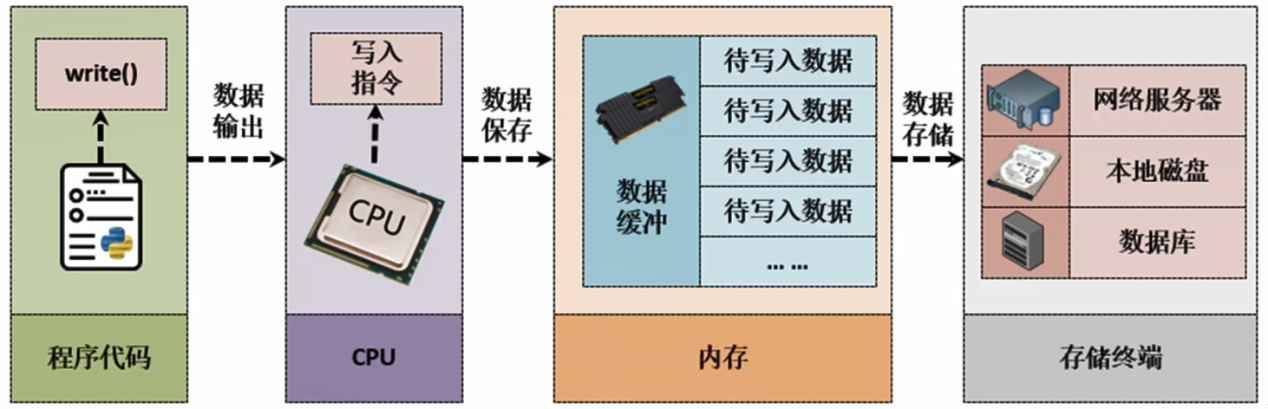
\includegraphics[scale=0.9]{img/C10/10-2/1.png}
	\caption{文件缓冲}
\end{figure}

开启缓冲可以提高写入效率,buffering参数设置有3种类型:

\begin{enumerate}
	\item 全缓冲(buffering > 1):当标准I/O缓存被填满后才会进行真正I/O操作,全缓冲的典型代表就是对磁盘文件的读写操作。

	\item 行缓冲(buffering = 1):在I/O操作中遇见换行符时才执行真正的I/O操作,例如在使用网络聊天工具时所编辑的文字在没有发送前是不会进行I/O操作的。

	\item 不缓冲(buffering = 0):直接进行终端设备的I/O操作,数据不经过缓冲保存。
\end{enumerate}

如果想要观察到行缓冲的使用特点,就不能直接使用with语句,因为with最后会执行close()的关闭操作,而一旦关闭,则缓冲的内容会全部进行输出。\\

使用flush()进行缓冲区的强制清空,一旦强制清空之后,缓冲区的内容将全部输出。每次使用close()关闭文件流的时候默认情况下也会调用flush()进行缓冲区的清空处理。\\

\mybox{文件缓冲}

\begin{lstlisting}[language=Python]
import os

def main():
    file = open(file="data.txt", mode="w",
                encoding="utf-8", buffering=1)
    file.write("This is a test.")
    os.system("pause")  # 程序暂停
    file.flush()        # 强制清空缓冲区
    os.system("pause")  # 程序暂停
    file.close()

if __name__ == "__main__":
    main()
\end{lstlisting}

\begin{tcolorbox}
	\mybox{运行结果}
	\textbf{data.txt}
	\begin{verbatim}
This is a test.
\end{verbatim}
\end{tcolorbox}

\newpage

\section{os模块}

\subsection{os模块}

os模块是Python用于与操作系统进行交互的一个操作模块,这个模块提供有大量与系统相关的处理函数,开发者可以直接通过Python程序进行操作系统的功能调用。

\begin{table}[H]
	\centering
	\setlength{\tabcolsep}{5mm}{
		\begin{tabular}{|l|l|}
			\hline
			\textbf{方法}     & \textbf{功能}      \\
			\hline
			getcwd()          & 获取当前的工作目录 \\
			\hline
			chdir(path)       & 修改工作目录       \\
			\hline
			system()          & 执行操作系统命令   \\
			\hline
			symlink(src, dst) & 创建软链接         \\
			\hline
			link(src, dst)    & 创建硬链接         \\
			\hline
		\end{tabular}
	}
	\caption{os模块}
\end{table}

\vspace{0.5cm}

\subsection{os.path子模块}

os.path是os模块之中的一个子模块,该子模块的核心作用在于进行路径处理操作。Python的程序代码本身是强调跨平台的,既然要进行跨平台的开发,尤其是在I/O路径的处理上就特别要引起注意。在Windows系统下路径分隔符使用的是【$ \backslash $】,而在Linux系统下使用的路径分隔符是【/】。所以在进行程序编写的时候就必须考虑到不同平台的设计问题。\\

使用os.path模块中提供的一系列函数可以针对给定的路径进行拆分处理以及判断和取得数据信息。\\

Python需要考虑不同操作系统的跨平台的特点,所以对于访问路径需要进行适当的变更,根据不同的操作系统使用不同的路径分隔符。如果每一次都判断操作系统就过于繁琐了,可以直接使用os.path中提供的变量来完成。

\begin{table}[H]
	\centering
	\setlength{\tabcolsep}{5mm}{
		\begin{tabular}{|c|l|}
			\hline
			\textbf{变量} & \textbf{功能}                                             \\
			\hline
			curdir        & 表示当前文件夹【.】,一般可以省略                         \\
			\hline
			pardir        & 上一层文件夹【..】                                        \\
			\hline
			sep           & 系统路径分隔符,Windows为【$ \backslash $】,Linux为【/】 \\
			\hline
			extsep        & 文件名称和后缀之间的间隔符【.】                           \\
			\hline
		\end{tabular}
	}
	\caption{路径分隔符}
\end{table}

\vspace{0.5cm}

\mybox{获取路径信息}

\begin{lstlisting}[language=Python]
import os

PATH = "code" + os.sep +"第10章 文件操作" + os.sep \
        + "10.3 os模块" + os.sep + "data.txt"

def main():
    if os.path.exists(PATH):
        print("绝对路径:%s" % os.path.abspath(PATH))
        print("文件名称:%s" % os.path.basename(PATH))
        print("文件大小:%s" % os.path.getsize(PATH))
        print("当前路径是否为文件:%s" % os.path.isfile(PATH))
        print("当前路径是否为目录:%s" % os.path.isdir(PATH))

if __name__ == "__main__":
    main()
\end{lstlisting}

\begin{tcolorbox}
	\mybox{运行结果}
	\begin{verbatim}
绝对路径:C:\Users\Administrator\Desktop\Python\code\第10章 文
件操作\10.3 os模块\data.txt
文件名称:data.txt
文件大小:15
当前路径是否为文件:True
当前路径是否为目录:False
\end{verbatim}
\end{tcolorbox}

\newpage

\section{csv模块}

\subsection{csv文件}

CSV (Comma-Separated Values,逗号分隔值/字符分隔值)是一种文件的格式,在该类型的文件里面一般会保存多个数据信息的内容,但是每一个数据信息一定都有各自的组成部分,用这样的文件进行数据采集内容的记录。CSV文件是跟人工智能和数据分析有直接联系的一种数据存储文件。\\

CSV是一种以纯文件方式进行数据记录的存储格式,在CSV文件内容使用不同的数据行记录数据的内容,每行数据使用特定的符号(一般是逗号)进行数据项的拆分,这样就形成了一种相对简单且通用的数据格式。在实际开发中利用CSV数据格式可以方便实现大数据系统中对于数据采集结果的信息记录,也可以方便进行数据文件的传输,同时CSV文件格式也可以被Excel工具所读取。\\

CSV文件是可以通过Excel工具打开的,当一个CSV文件被创建之后,在Windows系统中会自动和Excel软件进行关联。\\

\subsection{csv读写操作}

在Python中直接提供有csv模块,利用这个模块可以方便地实现数据的写入和读取操作,在CSV文件内容一般对于不同的数据项都要使用逗号分隔。除了数据之外,在CSV文件内容还可以设置文件标题。\\

\mybox{写入csv文件}

\begin{lstlisting}[language=Python]
import csv
import random

HEADER = ["Location", "Longitude", "Latitude"]

def main():
    # 如果不使用newline,那么每行记录之间就会多出一个空行
    with open(file="location.csv", mode="w", 
                newline="", encoding="utf-8") as file:
        csv_writer = csv.writer(file)       # 创建csv写入对象
        csv_writer.writerow(HEADER)         # 写入头部信息
        for i in range(1, 11):
            longitude = round(random.random() * 180, 3)   # [0, 180)
            latitude = round(random.random() * 90, 3)     # [0, 90)
            csv_writer.writerow(["loc-%d" % i, longitude, latitude])

if __name__ == "__main__":
    main()
\end{lstlisting}

\begin{tcolorbox}
	\mybox{运行结果}
	\textbf{location.csv}
	\begin{verbatim}
Location,Longitude,Latitude
loc-1,176.165,35.458
loc-2,12.729,56.247
loc-3,6.605,45.14
loc-4,15.123,53.435
loc-5,131.984,11.927
loc-6,155.038,35.681
loc-7,98.772,15.125
loc-8,70.991,30.328
loc-9,152.967,30.372
loc-10,96.362,76.798
\end{verbatim}
\end{tcolorbox}

\vspace{0.5cm}

\mybox{读取csv文件}

\begin{lstlisting}[language=Python]
import csv

def main():
    with open(file="location.csv", mode="r", 
                newline="", encoding="utf-8") as file:
        csv_reader = csv.reader(file)   # 创建csv读取对象
        header = next(csv_reader)       # 读取标题行
        print(header)
        for row in csv_reader:
            print(row)

if __name__ == "__main__":
    main()
\end{lstlisting}

\begin{tcolorbox}
	\mybox{运行结果}
	\begin{verbatim}
['Location', 'Longitude', 'Latitude']
['loc-1', '176.165', '35.458']
['loc-2', '12.729', '56.247']
['loc-3', '6.605', '45.14']
['loc-4', '15.123', '53.435']
['loc-5', '131.984', '11.927']
['loc-6', '155.038', '35.681']
['loc-7', '98.772', '15.125']
['loc-8', '70.991', '30.328']
['loc-9', '152.967', '30.372']
['loc-10', '96.362', '76.798']
\end{verbatim}
\end{tcolorbox}

\newpage

\section{pymysql模块}

\subsection{pymysql模块}

Python中针对MySQL数据库的开发操作提供有pymysql(Python3)和mysqldb(Python2)这两个核心模块。\\

对于数据库的开发操作,首先需要解决的就是数据库的连接。在Python中可以直接利用pymysql.connect()工厂函数获取数据库连接对象,这样就会返回一个pymysql.connections.Connection类的对象实例,通过此实例可以进行数据库的操作。\\

在进行connect()连接的时候必须明确地设置数据库连接的主机名称、端口号、用户名、密码、数据库名称。\\

\mybox{MySQL数据库操作}

\begin{lstlisting}[language=Python]
import pymysql
import traceback

INSERT = "INSERT INTO info VALUES \
            (3, 'Henry', 3.6)"
SEARCH = "SELECT * FROM info"

def main():
    try:
        # 连接数据库
        conn = pymysql.connect(
            host="localhost",
            port=3306,
            charset="UTF8",
            user="root",
            password="mysqladmin",
            database="student"
        )
        print("MySQL数据库连接成功")
        print("数据库版本:%s" % conn.get_server_info())

        db = conn.cursor()      # 获取数据库操作对象
        db.execute(INSERT)      # 执行SQL语句
        conn.commit()           # 提交事务,否则不会更新
        print("影响数据行数:%d" % db.rowcount)

        db.execute(SEARCH)
        for row in db.fetchall():   # 查询结果
            print(row)
    except Exception:
        print(traceback.format_exc())
    finally:
        db.close()

if __name__ == "__main__":
    main()
\end{lstlisting}

\begin{tcolorbox}
	\mybox{运行结果}
	\begin{verbatim}
MySQL数据库连接成功
数据库版本:8.0.26
影响数据行数:1
(1, 'Terry', 3.7)
(2, 'Lily', 4.2)
(3, 'Henry', 3.6)
\end{verbatim}
\end{tcolorbox}

\newpage